%%%%%%%%%%%%Outline%%%%%%%%%%%%%%%%%%

%%% Section 4 \tool: Extending the eBPF Compilation Pipeline

%%%
% message<\tool adds dual-form operations; constraints map to the subsections>
% \tool extends the pipeline with operations the verifier checks and the JIT emits
% each operation carries two forms, a proof sequence and a native emit
% the figure contrasts the pipeline with and without \tool
% a recognizer rewrites a pattern into extended instructions, each a pair of call and sidecar
% each call selects a descriptor from a kernel module, the descriptor supplies its two forms
% the same program verifies as vanilla eBPF and runs as native
% \tool meets the three constraints, each cashed by one subsection
% section 5 then presents \lang, the operations built with the mechanism

%%% Section 4.1 The Compilation Pipeline

%%%
% message<recognition turns idiom patterns into extended instructions without new opcodes>
% the recognizer matches the patterns of supported operations in userspace before load
% for \lang's rotate the pattern is the shift-and-or sequence
% the call and the sidecar reuse existing eBPF opcodes
% \tool therefore adds no new opcode

%%%
% message<the verifier checks an extended instruction by lowering it>
% the verifier checks an extended instruction by lowering it to vanilla eBPF
% the proof sequence is a vanilla eBPF fragment with the extended instruction's semantics
% a lowering stage substitutes the proof sequence before the main analysis
% the verifier analyzes the lowered program with its existing transfer functions
% after the analysis succeeds, a restore stage reinstates the extended instructions

%%%
% message<the JIT emits per-architecture native code; verification stays architecture-independent>
% the JIT dispatches each extended instruction to the descriptor's native emit
% for \lang's rotate, a single ROL on x86-64 or ROR on ARM64
% the exact proof sequence, like the native emit, can differ across architectures
% every proof-sequence variant stays vanilla eBPF
% verification therefore stays architecture-independent
% with no native emit the extended instruction falls back to the proof sequence
% the interpreter has no dispatch for extended instructions
% a kernel without a JIT therefore rejects programs that carry extended instructions

%%% Section 4.2 Adding an Operation

%%%
% message<a new operation is descriptors in a module plus a recognizer pattern>
% a new operation needs only descriptors in a kernel module and a pattern in the recognizer
% a descriptor is a small structure with two author-supplied parts, routine and emits
% a family of descriptors implements an operation, one per variant
% a kernel module registers its descriptors with the kernel core
% \tool's one-time core change stays the same for every operation

%%%
% message<an operation's size is open>
% the mechanism leaves an operation's size open
% a proof sequence may span a few instructions or an entire rule-conforming region

%%% Section 4.3 Safety and the Trusted Base

%%%
% message<the verification side adds nothing to the trusted base>
% the verification side adds nothing to the trusted computing base
% everything the recognizer and the module contribute reaches the verifier in the lowered program
% the verifier re-checks the lowered program on every load, same analysis as vanilla eBPF
% a faulty rewrite or proof sequence fails verification like any unsafe program

%%%
% message<the verdict carries over to the restored program>
% the verdict on the lowered program carries over to the restored program
% restore collapses each proof region back into its extended instruction, changes nothing else
% for the collapse to preserve the verdict, a region must stay single-entry, single-exit, jump-clean
% control enters a region only at its top and leaves only past its end, like one instruction
% at load time the kernel rejects calls, exits, or nesting inside a proof sequence
% the jump rules remain the operation author's responsibility

%%%
% message<the native emit is the sole evidence-owing addition>
% the native emit is the one component \tool adds to the trusted computing base
% the verifier never sees the native emit that the CPU runs
% every operation must supply evidence that its emit computes the same result as its proof sequence
% for \lang, the Lean 4 proofs supply the evidence

%%%%%%%%%%%%Outline%%%%%%%%%%%%%%%%%%

\section{\tool: Extending the eBPF Compilation Pipeline}
\label{sec:mechanism}
% \tool：扩展 eBPF 编译管线

\tool extends the eBPF compilation pipeline with new operations that the existing verifier checks and the kernel JIT emits directly.
% \tool 通过现有验证器检查且内核 JIT 直接发射的新操作来扩展 eBPF 编译管线。
Each operation has two forms: a \emph{proof sequence} of vanilla eBPF that the verifier checks and a \emph{native emit} that the CPU runs.
% 每个操作有两种形式：验证器检查的原生 eBPF \emph{证明序列}和 CPU 运行的\emph{本地发射}。
Figure~\ref{fig:pipeline} contrasts the pipeline with and without \tool.
% 图对比了有无 \tool 的管线。
A compile-time recognizer rewrites an operation's pattern into one or more \emph{extended instructions}, each a pair of a call and a sidecar that carries the operands.
% 编译时识别器将操作的模式重写为一条或多条\emph{扩展指令}，每条是一个调用和携带操作数的伴随对。
Each call selects a \emph{descriptor} from a kernel module, and the descriptor supplies both forms for its instruction.
% 每个调用从内核模块选择一个\emph{描述符}，描述符为其指令提供两种形式。
The same program therefore verifies as vanilla eBPF and runs as native code.
% 因此同一程序作为原生 eBPF 验证，作为本地代码运行。
\tool meets the three constraints of \S\ref{subsec:char-challenges}: the safety guarantee stays intact up to one explicit obligation (\S\ref{subsec:safety}), the kernel core changes once (\S\ref{subsec:adding}), and verification stays architecture-independent (\S\ref{subsec:pipeline}).
% \tool 满足三个约束：安全保证保持完整（有一个明确义务），内核核心只更改一次，验证保持架构无关。
\S\ref{sec:lang} then presents \lang, the hardware-idiom operations built with the mechanism.
% 接下来介绍用该机制构建的硬件习语操作 \lang。

\begin{figure*}[t]
\centering
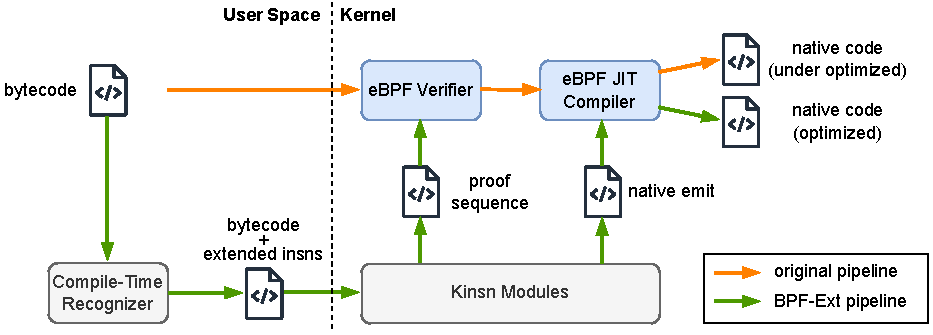
\includegraphics[width=0.9\textwidth]{figures/sec-4-pipeline-fig.pdf}
\caption{The original eBPF pipeline (orange) and the \tool pipeline (green). The original pipeline verifies and JIT-compiles the bytecode unchanged, producing under-optimized native code. With \tool, the compile-time recognizer rewrites supported operations into extended instructions, and the \lang modules supply each operation's proof sequence to the verifier and its native emit to the JIT, producing optimized native code.}
\label{fig:pipeline}
\end{figure*}

\subsection{The Compilation Pipeline}
\label{subsec:pipeline}
% 编译管线

\noindent\textbf{Recognition.}
% \noindent\textbf{识别。}
The recognizer matches the patterns of supported operations in userspace, before the program loads (\S\ref{subsec:llvm}).
% 识别器在程序加载前在用户空间匹配支持的操作模式。
For \lang's rotate, the pattern is the shift-and-or sequence of Figure~\ref{fig:jit-dump}.
% 对于 \lang 的旋转，模式是图中的移位与或序列。
The call and the sidecar reuse existing eBPF opcodes.
% 调用和伴随重用现有的 eBPF 操作码。
\tool therefore adds no new opcode.
% 因此 \tool 不添加新操作码。

\noindent\textbf{Verification.}
% \noindent\textbf{验证。}
The verifier checks an extended instruction by lowering it to vanilla eBPF.
% 验证器通过将扩展指令降低为原生 eBPF 来检查它。
The proof sequence is a fragment of vanilla eBPF with the same semantics as the extended instruction.
% 证明序列是具有与扩展指令相同语义的原生 eBPF 片段。
A lowering stage substitutes the proof sequence for the extended instruction before the main analysis.
% 降低阶段在主分析前用证明序列替换扩展指令。
The verifier then analyzes the lowered program with its existing transfer functions.
% 然后验证器用其现有的传递函数分析降低后的程序。
After the analysis succeeds, a restore stage reinstates the extended instructions for the JIT.
% 分析成功后，恢复阶段为 JIT 恢复扩展指令。

\noindent\textbf{Execution.}
% \noindent\textbf{执行。}
The JIT dispatches each extended instruction to the descriptor's native emit for the running architecture.
% JIT 将每条扩展指令分派到描述符对应运行架构的本地发射。
For \lang's rotate, the native emit is a single \texttt{ROL} on x86-64 or a single \texttt{ROR} on ARM64.
% 对于 \lang 的旋转，本地发射是 x86-64 上的单条 ROL 或 ARM64 上的单条 ROR。
The exact proof sequence, like the native emit, can differ across architectures.
% 确切的证明序列，像本地发射一样，可以在架构间不同。
Every proof-sequence variant stays vanilla eBPF.
% 每个证明序列变体都保持原生 eBPF。
Verification therefore stays architecture-independent.
% 因此验证保持架构无关。
When a descriptor provides no native emit for the architecture, the extended instruction falls back to its proof sequence, which the JIT compiles as vanilla eBPF.
% 当描述符不为该架构提供本地发射时，扩展指令回退到其证明序列，JIT 将其编译为原生 eBPF。
The interpreter has no dispatch for extended instructions.
% 解释器没有扩展指令的分派。
A kernel without a JIT therefore rejects programs that carry extended instructions.
% 因此没有 JIT 的内核会拒绝携带扩展指令的程序。

\subsection{Adding an Operation}
\label{subsec:adding}
% 添加操作

A new operation needs only descriptors in a kernel module and a pattern in the recognizer.
% 新操作只需要内核模块中的描述符和识别器中的模式。
A descriptor is a small kernel structure with two author-supplied parts, the proof-sequence routine and the per-architecture native emits.
% 描述符是一个小的内核结构，有两个作者提供的部分：证明序列例程和每架构本地发射。
A family of descriptors implements an operation, one descriptor per variant, such as width, condition, or architecture.
% 一系列描述符实现一个操作，每个变体一个描述符，如宽度、条件或架构。
A kernel module registers its descriptors with the kernel core.
% 内核模块向内核核心注册其描述符。
\tool's one-time change to the kernel core stays the same for every operation (\S\ref{sec:implementation}).
% \tool 对内核核心的一次性更改对每个操作保持相同。

The mechanism leaves an operation's size open.
% 该机制对操作的大小开放。
A proof sequence may span a few instructions or an entire region within the rules of \S\ref{subsec:safety}.
% 证明序列可以跨越几条指令或在规则内的整个区域。

\subsection{Safety and the Trusted Base}
\label{subsec:safety}
% 安全性与可信基

\tool does not add operation-specific abstract semantics to the verifier.
% \tool 不向验证器添加操作特定的抽象语义。
Everything the recognizer and the module contribute reaches the verifier inside the lowered program.
% 识别器和模块贡献的一切都在降低后的程序内到达验证器。
The verifier re-checks the lowered program on every load, with the same analysis as for vanilla eBPF.
% 验证器在每次加载时重新检查降低后的程序，使用与原生 eBPF 相同的分析。
A faulty rewrite or proof sequence that violates safety therefore fails verification like any unsafe program.
% 因此违反安全的错误重写或证明序列会像任何不安全程序一样验证失败。

The verifier's verdict on the lowered program carries over to the restored program.
% 验证器对降低后程序的裁决传递到恢复后的程序。
The restore stage collapses each \emph{proof region}, the span its proof sequence occupies, back into its extended instruction and changes nothing else.
% 恢复阶段将每个\emph{证明区域}（其证明序列占据的范围）折叠回其扩展指令，其他不变。
For the collapse to preserve the verdict, a region must stay single-entry and single-exit, free of nested extended instructions, calls, exits, and backward jumps.
% 为使折叠保持裁决，区域必须保持单入口单出口，没有嵌套扩展指令、调用、退出和向后跳转。
Control then enters a region only at its top and leaves only past its end, like a single instruction.
% 然后控制只从区域顶部进入，只从末尾之后离开，像单条指令。
The kernel validates proof-region well-formedness at load time, including single entry, single exit, no nested extended instructions, and no calls or exits inside a region.
% 内核在加载时验证证明区域的良构性，包括单入口、单出口、无嵌套扩展指令、区域内无调用或退出。
The kernel also validates that no jump enters or leaves a region except at its boundary.
% 内核还验证除边界外没有跳转进入或离开区域。

The trusted enforcement path therefore consists of the existing eBPF verifier and JIT plus a small, generic \tool patch that validates proof regions, lowers extended instructions before verification, restores them after verification, and dispatches their native emits (\S\ref{sec:implementation}).
% 因此可信执行路径包括现有的 eBPF 验证器和 JIT，加上一个小的通用 \tool 补丁，用于验证证明区域、在验证前降低扩展指令、在验证后恢复它们、并分派它们的本地发射。
The per-operation native emit is the one component whose correctness \tool cannot check at load time.
% 每操作本地发射是 \tool 无法在加载时检查其正确性的唯一组件。
Every operation must therefore supply evidence that its native emit has the same eBPF-visible effect as its proof sequence.
% 因此每个操作必须提供证据，证明其本地发射具有与其证明序列相同的 eBPF 可见效果。
For \lang, the Lean 4 proofs of \S\ref{sec:formal-verification} supply the evidence.
% 对于 \lang，Lean 4 证明提供了证据。
The userspace recognizer is outside the safety boundary: an incorrect rewrite produces a program the verifier re-checks and rejects or accepts on its own merits.
% 用户空间识别器在安全边界之外：不正确的重写产生的程序由验证器重新检查并根据其本身优劣拒绝或接受。